\subsection{Физические модели фотоиндуцированной генерации второй гармоники в оптических волокнах}\label{subsec:dianov_antonyuk}

\subsubsection{Ориентационные и зарядовые модели}

Все предложенные для объяснения фотоиндуцированной ГВГ модели можно разделить на два класса: ориентационные и зарядовые~\cite{dianov1995photoinduced}. 

\begin{figure}[h]
	\centering
	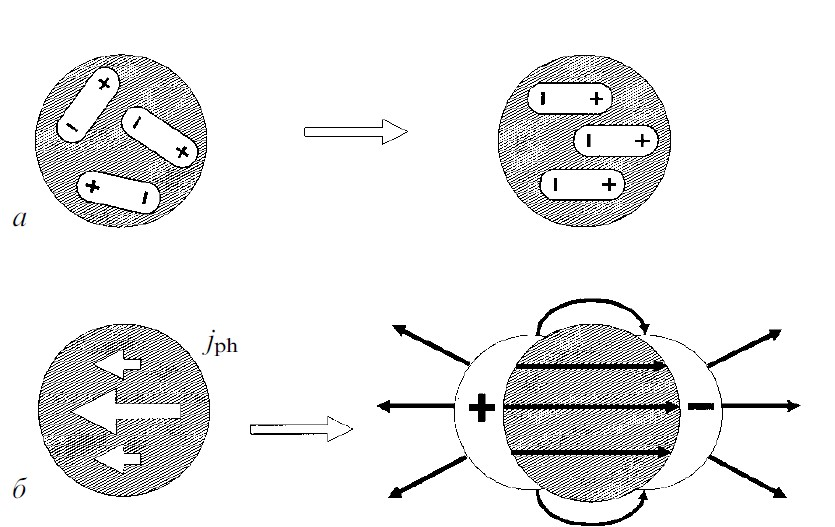
\includegraphics[width=0.55\linewidth]{Dissertation/images/review/models}
	\caption{Возникновение фотоиндуцированного электрического поля в ориентационных (а) и зарядовых (б) моделях}
	\label{fig:models}
\end{figure}


В ориентационных моделях (рис.~\cref{fig:models}, а)) предполагается, что асимметрия на микроскопическом уровне уже существует в виде хаотически ориентированных дипольных моментов (асимметричные молекулы, дефекты структуры). Под действием света происходит упорядочивание хаотически расположенных диполей:

\begin{equation}
	\mathbf{D} = \sum_i \mathbf{d}_i.
\end{equation}

В зарядовых моделях (рис.~\ref{fig:models}, б) предполагается, что под действием лазерного излучения происходит фотоионизация зарядов, макроскопическое их разделение и формирование постоянного электрического поля $E_{dc}$, которое через кубическую нелинейность индуцирует квадратичную восприимчивость:

\begin{equation}
	\chi^{(2)} = 3\chi^{(3)} E_{dc}.
\end{equation}

Важное отличие двух моделей заключается в характерных размерах области с ненулевым электрическим полем: в ориентационных моделях эта область сопоставима по размеру со световым пятном, в то время как в зарядовых моделях силовые линии электростатического поля простираются значительно дальше освещённой области (см.~\cref{fig:models}).

На основе накопленных экспериментальных данных были предложены две детальные микроскопические модели, объясняющие формирование решётки $\chi^{(2)}$: фотогальваническая модель Дианова и Стародубова~\cite{dianov1995photoinduced} и модель самоорганизации экситонов с переносом заряда Б.~Антонюка и В.~Антонюка~\cite{antonyuk2001self}. Обе модели относятся к классу зарядовых в том смысле, что связывают возникновение $\chi^{(2)}$ с наличием статического электрического поля $E_{dc}$. Однако они предлагают принципиально разные механизмы возникновения и усиления этого поля. Модель Антонюка, формально являясь ориентационной, включает положительную обратную связь, что принципиально отличает её от классических ориентационных моделей типа Столена--Тома. Ниже эти модели рассмотрены подробно, а затем приведены экспериментальные факты, которые каждая из них объясняет.


\subsubsection{Модель когерентного фотогальванического фотоэффекта}\label{subsubsec:dianov}
\nomenclature{КФЭ}{Когенертный фотогальванический эффект}


\subsubsection{Модель самоорганизации экситонов с переносом заряда}\label{subsubsec:antonyuk}
\nomenclature{ЭПЗ}{Экситоны с переносом заряда}


%Эксперимент, позволивший разделить два механизма, был проведён в 1992 году \cite{djanov1992photo}. Советский и российский учёный Евгений Дианов c коллегами предложили методику, основанную на существенной роли границы освещаемой области: при изменении граничного заряда в рамках зарядовой модели распределение электрического поля изменится значительно, а в рамках ориентационной~--- слабо. Из-за этого при смещении освещаемой области вдоль направления разделения зарядов представляется возможным создать протяжённую область заряда одного знака и малую~--- другого. При этом будут наблюдаться три максимума электрического поля (рис. \ref{fig:expsplit}, слева) и, как следствие, три максимума эффективности генерации гармоники. При движении в перпендикулярном направлении, равно как при работе в рамках ориентационной модели, зарядовые области будут одного размера и область эффективной генерации также будет однородной. Эксперимент подтвердил предположения авторов (рис. \ref{fig:expsplit}, справа)), и зарядовые модели стали доминирующими среди прочих предлагаемых физических механизмов генерации второй гармоники в оптическом волокне.
%
%\begin{figure}
%	\centering
%	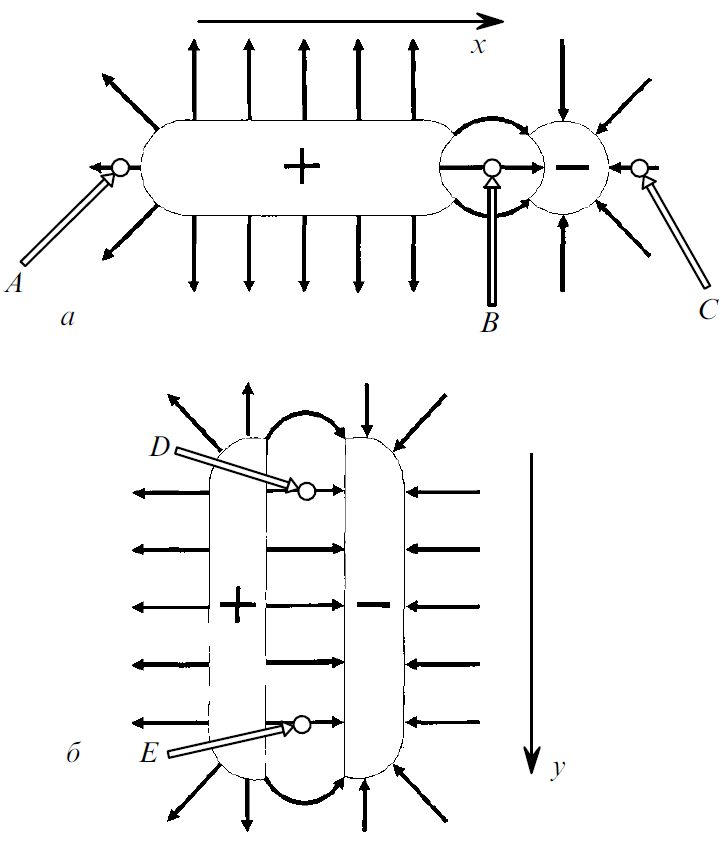
\includegraphics[width=0.5\linewidth]{Dissertation/images/review/expSplit.jpg}
%	\caption{Слева: распределение электрического поля в зарядовой модели при движении пятна света параллельно (а) и перпендикулярно (б) направлению разделения зарядов. Справа: мощность второй гармоники при движении в соответствующих направлениях}
%	\label{fig:expsplit}
%\end{figure}
%
%
%На основании проведённой работы коллектив Диановского волоконного центра предложил и развил зарядовую модель, основанную на анизотропном когерентном фотовольтаическом эффекте \cite{dianov1995photoinduced}.
%
%
%%Как отмечалось в главе про волокно, для достижения волноводного эффекта в световодах посредством увеличения показателя преломления сердцевины волокна необходимо добавлять в плавленый кварц соответствующие примеси. Именно они и являются источником дефектов, приводящих в конечном счёте к фотоиндуцированной генерации второй гармоники.
%%

%В 2000 году была предложена физическая модель, объединяющая зарядовые и ориентационные особенности предыдущих моделей \cite{antonyuk2001self}. Проводя анализ спектров комбинационного, гиперкомбинационного и люминесцентного спектра оптического волокна, легированного оксидом германия, авторы предложили модель усиления слабого затравочного поля, основанную на самоорганизации возбуждений в среде. Согласно этой модели, примесный электрон, находящийся на Ge-центре поглощает один квант волны второй гармоники (зелёный свет) и переходит либо на другой Ge-центр, либо в силикатную матрицу.  Создаётся \textsf{экситон с переносом заряда (ЭПЗ)}, представляющий собой электрический диполь. Рассматривая электрон-дырочную кинетику в среде, авторы пришли к выводу, что экситоны с переносом заряда представляют собой систему с обратной положительной связью и ориентируются в слабом постоянном электрическом поле так, чтобы его усилить до величины $E\approx10^5~\text{В}/\text{см}$.
%%
%Далее авторы объединяют свою модель с уже существующими, рассматривая усиление слабой волны второй гармоники в периодическом (по длине) электрическом поле, созданным экситонами с переносом заряда. Учёт истощения накачки приводит к первому в мире правильному объяснению временной зависимости эффективности генерации, а также резкому увеличению мощности с последующим спадом при изменении фазовых соотношений между волнами накачки и второй гармоники.
%
%Представим изложенную логику генерации второй гармоники в виде схемы:
%\begin{figure}[h]
%	\centering
%	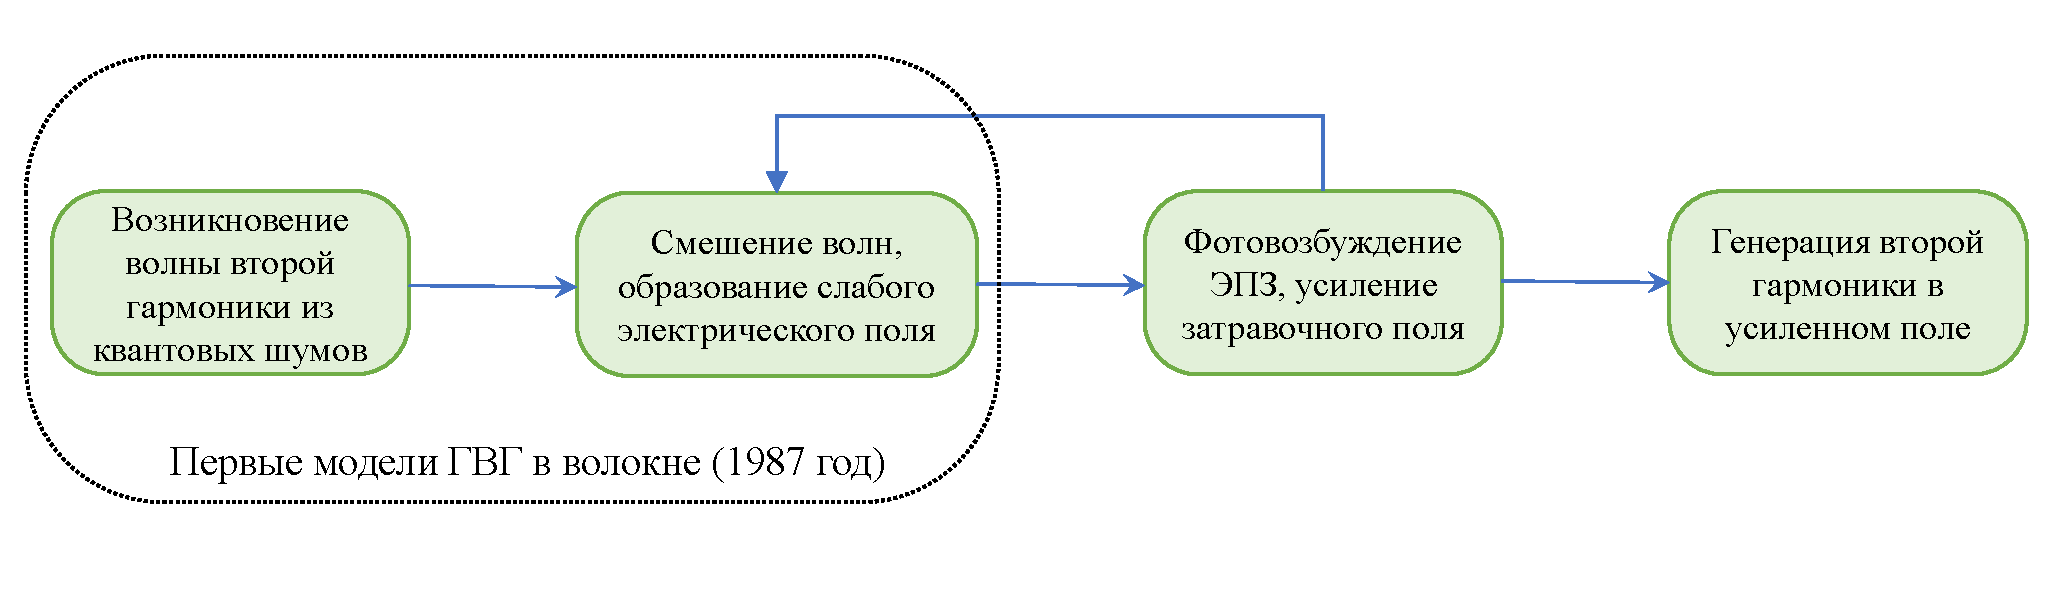
\includegraphics[width=0.99\linewidth]{Dissertation/images/review/scheme_epz}
%	\caption{Упрощённая схема физических процессов при генерации второй гармоник в волокне согласно \cite{antonyuk2001self}}
%	\label{fig:schemeepz}
%\end{figure}
%Как следует из схемы, изображённой на рис. \ref{fig:schemeepz}, в предложенной автором модели находят отражение первые теоретические объяснения эффекта, изложенные сразу после его экспериментального наблюдения.
